% log10 of the error of Stirling's series for log Gamma(x) with m terms, x = 1, 2, 4. Generated by a short script.
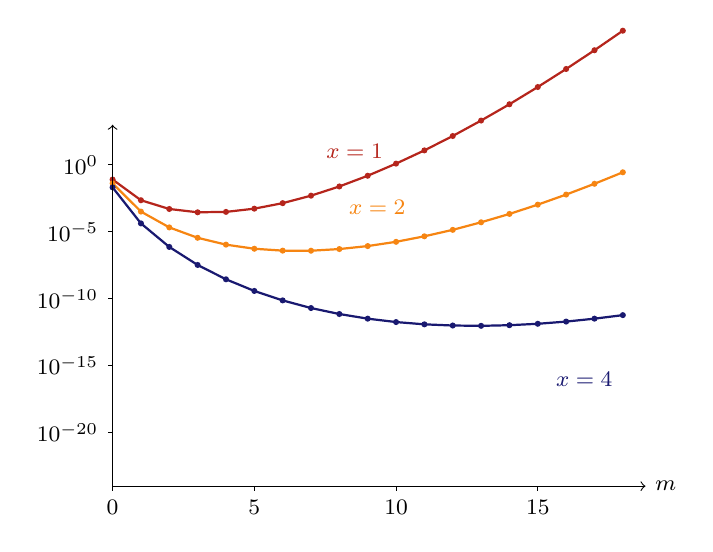
\begin{tikzpicture}[every node/.style={font=\footnotesize}]
\draw[BrickRed,thick] (0.000,3.894)--(0.360,3.631)--(0.720,3.520)--(1.080,3.478)--(1.440,3.483)--(1.800,3.524)--(2.160,3.594)--(2.520,3.689)--(2.880,3.806)--(3.240,3.942)--(3.600,4.096)--(3.960,4.264)--(4.320,4.447)--(4.680,4.643)--(5.040,4.850)--(5.400,5.069)--(5.760,5.298)--(6.120,5.536)--(6.480,5.784);
\fill[BrickRed] (0.000,3.894) circle (1.1pt);
\fill[BrickRed] (0.360,3.631) circle (1.1pt);
\fill[BrickRed] (0.720,3.520) circle (1.1pt);
\fill[BrickRed] (1.080,3.478) circle (1.1pt);
\fill[BrickRed] (1.440,3.483) circle (1.1pt);
\fill[BrickRed] (1.800,3.524) circle (1.1pt);
\fill[BrickRed] (2.160,3.594) circle (1.1pt);
\fill[BrickRed] (2.520,3.689) circle (1.1pt);
\fill[BrickRed] (2.880,3.806) circle (1.1pt);
\fill[BrickRed] (3.240,3.942) circle (1.1pt);
\fill[BrickRed] (3.600,4.096) circle (1.1pt);
\fill[BrickRed] (3.960,4.264) circle (1.1pt);
\fill[BrickRed] (4.320,4.447) circle (1.1pt);
\fill[BrickRed] (4.680,4.643) circle (1.1pt);
\fill[BrickRed] (5.040,4.850) circle (1.1pt);
\fill[BrickRed] (5.400,5.069) circle (1.1pt);
\fill[BrickRed] (5.760,5.298) circle (1.1pt);
\fill[BrickRed] (6.120,5.536) circle (1.1pt);
\fill[BrickRed] (6.480,5.784) circle (1.1pt);
\draw[BurntOrange,thick] (0.000,3.845)--(0.360,3.487)--(0.720,3.286)--(1.080,3.154)--(1.440,3.067)--(1.800,3.015)--(2.160,2.991)--(2.520,2.990)--(2.880,3.011)--(3.240,3.049)--(3.600,3.103)--(3.960,3.173)--(4.320,3.255)--(4.680,3.351)--(5.040,3.457)--(5.400,3.575)--(5.760,3.703)--(6.120,3.840)--(6.480,3.986);
\fill[BurntOrange] (0.000,3.845) circle (1.1pt);
\fill[BurntOrange] (0.360,3.487) circle (1.1pt);
\fill[BurntOrange] (0.720,3.286) circle (1.1pt);
\fill[BurntOrange] (1.080,3.154) circle (1.1pt);
\fill[BurntOrange] (1.440,3.067) circle (1.1pt);
\fill[BurntOrange] (1.800,3.015) circle (1.1pt);
\fill[BurntOrange] (2.160,2.991) circle (1.1pt);
\fill[BurntOrange] (2.520,2.990) circle (1.1pt);
\fill[BurntOrange] (2.880,3.011) circle (1.1pt);
\fill[BurntOrange] (3.240,3.049) circle (1.1pt);
\fill[BurntOrange] (3.600,3.103) circle (1.1pt);
\fill[BurntOrange] (3.960,3.173) circle (1.1pt);
\fill[BurntOrange] (4.320,3.255) circle (1.1pt);
\fill[BurntOrange] (4.680,3.351) circle (1.1pt);
\fill[BurntOrange] (5.040,3.457) circle (1.1pt);
\fill[BurntOrange] (5.400,3.575) circle (1.1pt);
\fill[BurntOrange] (5.760,3.703) circle (1.1pt);
\fill[BurntOrange] (6.120,3.840) circle (1.1pt);
\fill[BurntOrange] (6.480,3.986) circle (1.1pt);
\draw[MidnightBlue,thick] (0.000,3.794)--(0.360,3.337)--(0.720,3.038)--(1.080,2.809)--(1.440,2.627)--(1.800,2.479)--(2.160,2.359)--(2.520,2.262)--(2.880,2.186)--(3.240,2.127)--(3.600,2.084)--(3.960,2.055)--(4.320,2.040)--(4.680,2.036)--(5.040,2.044)--(5.400,2.062)--(5.760,2.090)--(6.120,2.127)--(6.480,2.172);
\fill[MidnightBlue] (0.000,3.794) circle (1.1pt);
\fill[MidnightBlue] (0.360,3.337) circle (1.1pt);
\fill[MidnightBlue] (0.720,3.038) circle (1.1pt);
\fill[MidnightBlue] (1.080,2.809) circle (1.1pt);
\fill[MidnightBlue] (1.440,2.627) circle (1.1pt);
\fill[MidnightBlue] (1.800,2.479) circle (1.1pt);
\fill[MidnightBlue] (2.160,2.359) circle (1.1pt);
\fill[MidnightBlue] (2.520,2.262) circle (1.1pt);
\fill[MidnightBlue] (2.880,2.186) circle (1.1pt);
\fill[MidnightBlue] (3.240,2.127) circle (1.1pt);
\fill[MidnightBlue] (3.600,2.084) circle (1.1pt);
\fill[MidnightBlue] (3.960,2.055) circle (1.1pt);
\fill[MidnightBlue] (4.320,2.040) circle (1.1pt);
\fill[MidnightBlue] (4.680,2.036) circle (1.1pt);
\fill[MidnightBlue] (5.040,2.044) circle (1.1pt);
\fill[MidnightBlue] (5.400,2.062) circle (1.1pt);
\fill[MidnightBlue] (5.760,2.090) circle (1.1pt);
\fill[MidnightBlue] (6.120,2.127) circle (1.1pt);
\fill[MidnightBlue] (6.480,2.172) circle (1.1pt);
\draw[->] (0,0)--(6.768,0) node[right] {$m$};
\draw[->] (0,0)--(0,4.590);
\draw (0,0.680)--(-0.06,0.680) node[left] {$10^{-20}$};
\draw (0,1.530)--(-0.06,1.530) node[left] {$10^{-15}$};
\draw (0,2.380)--(-0.06,2.380) node[left] {$10^{-10}$};
\draw (0,3.230)--(-0.06,3.230) node[left] {$10^{-5}$};
\draw (0,4.080)--(-0.06,4.080) node[left] {$10^{0}$};
\draw (0.000,0)--(0.000,-0.06) node[below] {$0$};
\draw (1.800,0)--(1.800,-0.06) node[below] {$5$};
\draw (3.600,0)--(3.600,-0.06) node[below] {$10$};
\draw (5.400,0)--(5.400,-0.06) node[below] {$15$};
\node[BrickRed,right] at (2.592,4.250) {$x=1$};
\node[BurntOrange,right] at (2.880,3.536) {$x=2$};
\node[MidnightBlue,right] at (5.508,1.360) {$x=4$};
\end{tikzpicture}
